\subsubsection{UC6 - Gestione carrello}
 \begin{figure}[h]
	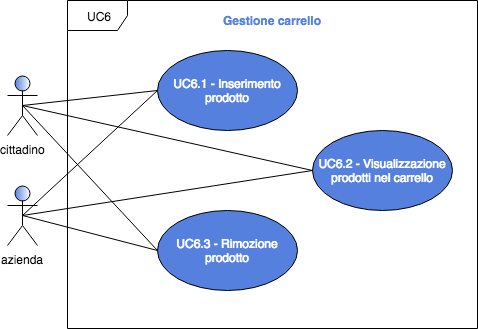
\includegraphics[width=6cm]{res/images/UC6GestioneCarrello.png}
	\centering
	\caption{UC6 - Gestione carrello}
\end{figure}
\begin{itemize}
	\item \textbf{Attori Primari}: cittadino, azienda\glo;
	\item \textbf{Descrizione}: l'utente, che sia esso cittadino o azienda, ha il totale controllo del proprio carrello, con possibilità di aggiunta e rimozione di beni e/o servizi, con possibilità di trarne un riepilogo;
	\item \textbf{Scenario principale}: l'utente effettua le operazioni necessarie all'acquisto di beni e servizi. Esse comprendono:
	\begin{enumerate}[label=\alph*.]
		\item l'inserimento di un bene/servizio [UC6.1];
		\item la visualizzazione dei prodotti nel carrello [UC6.2];
		\item la rimozione di prodotto dal carrello [UC6.3];
	\end{enumerate}
	\item \textbf{Precondizione}: l'utente necessita di acquistare un prodotto o un servizio;
	\item \textbf{Postcondizione}: l'utente può procedere all'acquisto di tutti i beni e/o servizi presenti nel carrello.
\end{itemize} 
 \subsubsection{UC6.1 - Inserimento prodotto}
\begin{itemize}
	\item \textbf{Attori Primari}: cittadino, azienda\glo;
	\item \textbf{Descrizione}: l'utente inserisce il prodotto selezionato nel carrello, nella quantità desiderata;
	\item \textbf{Scenario principale}:
	\begin{enumerate}[label=\alph*.]
		\item l'utente sta visualizzando i prodotti offerti [UC5];
		\item l'utente seleziona la quantità desiderata del prodotto [UC5.1];
		\item l'utente preme il pulsate per l'inserimento del prodotto nel carrello;
	\end{enumerate}
	\item \textbf{Precondizione}: l'utente deve poter visualizzare i beni/servizi ed esprime la volontà di inserire un prodotto nel carrello premendo l'apposito pulsante;
	\item \textbf{Postcondizione}: nel carrello dell'utente è presente il bene o il servizio selezionato.
\end{itemize}
\subsubsection{UC6.2 - Visualizzazione prodotti del carrello}
\begin{itemize}
	\item \textbf{Attori Primari}: cittadino, azienda\glo;
	\item \textbf{Descrizione}: l'utente visualizza un riepilogo di tutti i prodotti presenti all'interno el proprio carrello. Per ognuno di essi può visualizzare dei dettagli riassuntivi, che sono:
	\begin{itemize}
		\item nome;
		\item prezzo; 
		\item quantità;
	\end{itemize}
	\item \textbf{Scenario principale}: l'utente si trova all'interno della pagina del proprio carrello virtuale e può visualizzare la lista dei prodotti aggiunti al carrello;
	\item \textbf{Precondizione}: l'utente deve essere all'interno della pagina del proprio carrello;
	\item \textbf{Postcondizione}: l'utente ha potuto controllare la lista dei prodotti all'interno del proprio carrello.
\end{itemize}
\subsubsection{UC6.3 - Rimozione prodotto}
\begin{itemize}
	\item \textbf{Attori Primari}: cittadino, azienda\glo;
	\item \textbf{Descrizione}: l'utente rimuove il prodotto selezionato dal proprio carrello;
	\item \textbf{Scenario principale}: l'utente si trova all'interno del carrello e clicca sul pulsante dedicato alla rimozione dello stesso dal carrello virtuale;
	\item \textbf{Precondizione}: l'utente deve essere all'interno della pagina del proprio carrello;
	\item \textbf{Postcondizione}: nel carrello dell'utente non vi è più presente il bene o il servizio rimosso.
\end{itemize}